\chapter*{Prototipo}
\chaptermark{Prototipo}
\addcontentsline{toc}{chapter}{Prototipo}

In questo capitolo, presenteremo le parti significative di un prototipo di applicazione che utilizza il protocollo RLN e la tecnologia zk\_SNARK  per applicare una regola di limitazione della velocità in un sistema centralizzato, dove Client e Server interagiscono in completo anonimato.

Al fine di concentrarci sulle dinamiche del protocollo per comprenderne il funzionamento, ho scelto di semplificare la parte strutturale del prototipo, che è composta da un Server che espone un servizio di registrazione e di interazione, e alcuni Client che comunicano con il Server attraverso un canale di comunicazione basato su socket.

Si tenga presente che il protocollo non ha pretese di essere un progetto realmente funzionante, ma piuttosto di essere un utile strumento per coloro che desiderano acquisire familiarità con le tecnologie zero knowledge e applicarle concretamente. Ciò nonostante sarà possibile valutare i benefici e le criticità che queste tecnologie portano in campo, mediante il calcolo delle prestazioni e l'analisi del codice.

\section{Tecnologie e struttura}
Per lo sviluppo del prototipo, ho attuato la scelta di utilizzare il linguaggio di programmazione TypeScript. Questa decisione è stata presa in considerazione delle specifiche necessità del progetto, e in particolare delle librerie sviluppate e attive per la tecnologia zk-SNARK e per il protocollo RLN. La struttura del progetto è un monorepo (unica repository con molteplici progetti) che contiene sia i dati e il codice del Server che quelli reltiva al Client. Entrambi i componenti, utilizzano Node.js come ambiente di esecuzione. Infatti dopo la compilazione del codice TypeScript in JavaScript, il codice viene eseguito tramite il runtime Node.js. 
Le librerie utilizzate sono le seguenti:
\begin{itemize}
    \item \textbf{Circom 2}: usata per la generazione e la compilazione dei circuiti del progetto. Circom consiste di un compilatore Rust per i circuiti scritti l'inguaggio circom (omonimo della libreria). Inotre comprende anche diversi template di circuiti che assolvono specifiche funzioni molto utli come l'implementazione della funzione di hash Poseidon.
    \item \textbf{Socket.IO}: è una libreria JavaScript che consente di creare e gestire connessioni in tempo reale tra il Client e il Server. Si basa sul protocollo WebSocket e permette di creare una comunicazione bidirezionale tra il Client e il Server implementando anche un sistema basato sugli eventi, ispirato alla classe EventEmitter di Node.js
    \item \textbf{RLN Circuits}: in questa libreria sono preseti i circuiti che implementano le funioni principarli del protocollo RLN. In particolare, sono presenti i circuiti per la registrazione, la verifica, la punizione e alcuni circuiti di supporto.
    \item \textbf{RLNjs}: è una libreria scritta in TypeScript che implementa la logica del protocollo RLN. Sfrutta i circuiti messi a disposizione dalla libreria precedente per implementare la logica di verifica e generazione delle prove.
\end{itemize}

Inoltre ho utilizzato il package manager ufficiale di Node.js, npm, per installare rapidamente e facilmente le librerie e i moduli di cui hai avuto bisogno e Eslint uno strumento di analisi del codice statico che aiuta a individuare e correggere errori e eventuali vulnerabilità del codice.

\section{Circuiti}
Come spiegato nella sezione relativa alla proprietà succint di zk-SNARK per potre creare un programma che usi questa tecnologia, abbiamo bisogno di formulare le porzioni di logica del programma che vogliamo provare (dimostrare) attraverso dei circuiti algebrici. Le parti significative del codice di cui vogliamo creare una Zero Knowledge Proof sono l'appartenzenza all'albero di Merkle e la corretta costruzione delle porzione di segreto che ogni Client rilascia al Server durante l'interazione. Per questo motivo abbiamo bisogno di due circuiti:
\begin{enumerate}
    \item \textbf{proof of membership}:
    \begin{figure}[H]
        \centering
        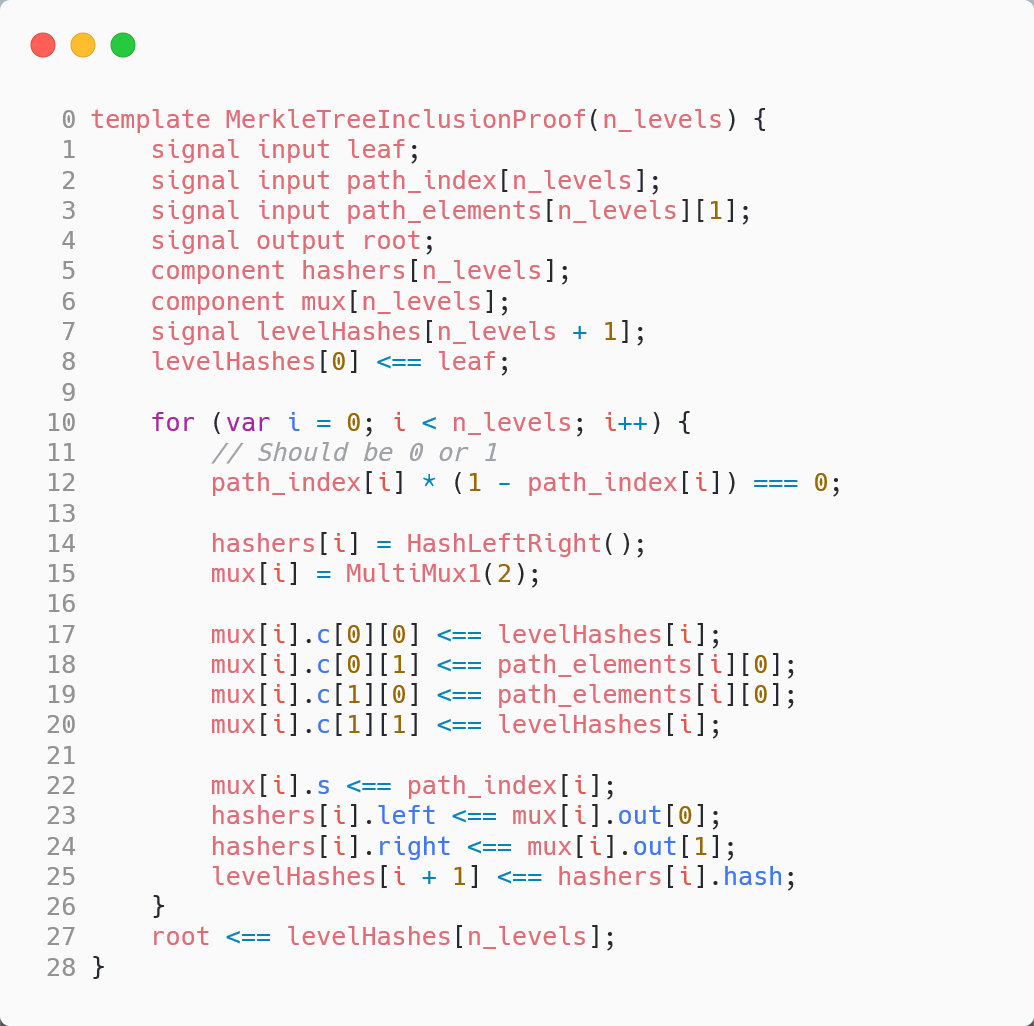
\includegraphics[width=10cm]{./chapters/3.poc/images/1.merkle_proof.png}
        \label{fig:merkle_proof}
        \captionsetup{justification=centering}
        \caption{codice circuito proof of membership}
    \end{figure}
    Nel codice in figura possiamo vedere il circuito scritto in codice circom che implementa la ricerca di un elemento all'interno di un albro di Merkle, il circuito prende in ingresso tre paramentri: la prfonditò dell' albero, il valore della foglia da cercare, il percorso binario, dove 0 indica il ramo di sinistra e 1 indica il ramo di destra, che bisogna seguire partendo dalla radice per raggiungere la foglia e le altre foglie dell'albero. Il circuito restiturisce la radice dell'albero. I componenti $HashLeftRight()$ e $MultiMux1()$ sono due componenti ausiliari che servono rispettivamente a apllicare la funzione hash ai nodi figli e a selezionare i nodi corretti in base al livello dell'albero in cui ci troviamo.
    \item \textbf{verifica delle porzioni del segreto}:
    \begin{figure}[H]
        \centering
        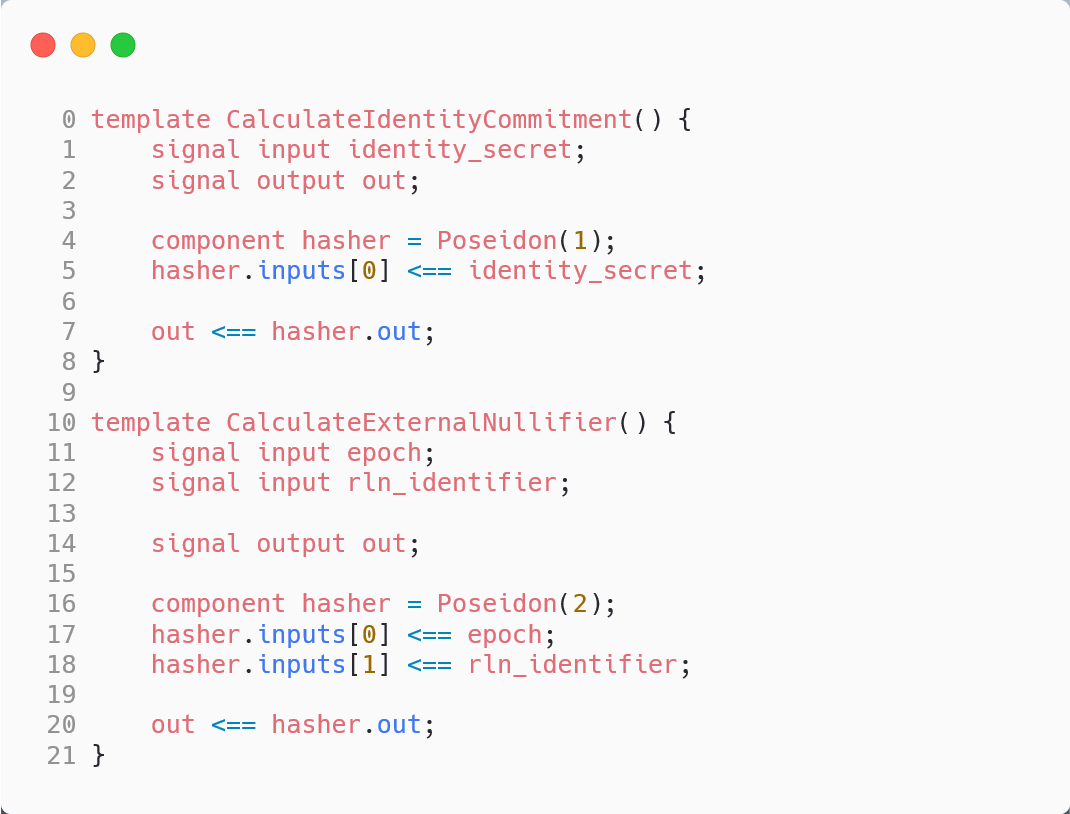
\includegraphics[width=11cm]{./chapters/3.poc/images/2.1.verify_shares.png}
        \label{fig:1.verify_shares}
        \captionsetup{justification=centering}
        \caption{codice circuito proof of membership}
    \end{figure}
    In questa prima porzione di codice possiamo vedere due funzioni fondamentali del protocollo RLN, ovvero la funzione $CalculateIdentityCommitment()$ che permette di verificare che l'identity commitment venga effettivamente calcolato a partire dalla chiave privata e $CalculateExternalNullifier()$ che è quel circuito ci permette di ottenere un nullifiere diverso per singolo mesaggio.\clearpage
    \begin{figure}[H]
        \centering
        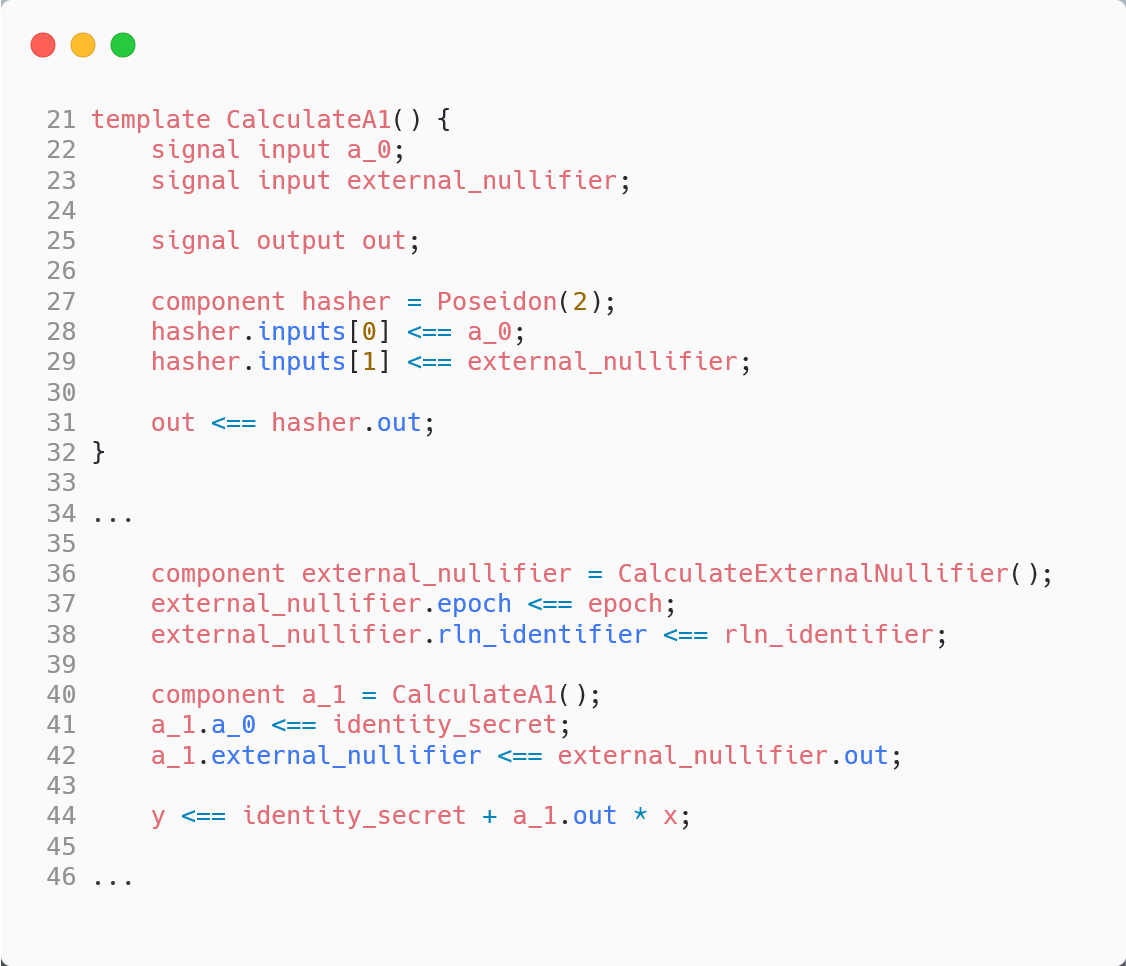
\includegraphics[width=11cm]{./chapters/3.poc/images/2.2.verify_shares.png}
        \label{fig:2.verify_shares}
        \captionsetup{justification=centering}
        \caption{codice circuito proof of membership}
    \end{figure}
    Mentre in questa porzione vediamo ancora una funzione atomica ovvero CalculateA1() che permette di ottenere il valore a1 che fa variare il polinomio di verifica a seconda dell' external\_nullifier e della chiave privata seguendo la formula vista in precedenza $a_1 = Poseidon(a_0, externalNullifier)$ e in fine vediamo una porzione di codice dove tutte le funzioni precedenti vengono utilizzate per verificare che il segreto sia stato costruito correttamente.
\end{enumerate}

Ricordo che il codice visto fino ad adesso non rappresenta la logica del protocollo ma solamente, i circuiti algebrici che verranno trasformati in vincoli per la verifica che il Client soddisfi e rispetti pur rimanendo anonimo le regole del servizio.

Per ottenere i file che verranno utilizzati da Server e Client per provare e verificare le dimostazione, bisogna compilare i circuiti utilizzando circom. Alla fine della fase di compilazione che si divide in trasformazione da circuito a QAP e successiva fase di trustedSetup che ovviamente in questo caso è stat svolta con un unico partecipantem, otteniamo i seguenti file:
\begin{itemize}
    \item \textbf{rln\_final.zkey}: file che contiene i parametri crittografici e i paramentri privati che consentono a un verificatore di controllare la validità di una prova senza rivelare alcuna informazione sui dati sottostanti.
    \item \textbf{rln.wasm}: è una versione compilata del circuito che può essere eseguita in un browser web utilizzando WebAssembly. Questo file è generato dal codice Circom e contiene la logica del circuito in un formato binario che può essere eseguito.
    \item \textbf{verification\_key.json}: contiene una chiave pubblica relativa al circuito, che può essere usata da un verificatore per controllare la validità di una prova.
\end{itemize}

\section{Server}
La struttura del Server è semplice: si tratta di un progetto Node.js che utilizza la libreria Socket.IO per gestire la comunicazione con i Client. Il Server è composto da due classi principali: "server.ts" e "type.ts". La prima classe contiene la logica applicativa e implementa le primitive della libreria RLNjs per verificare le prove dei Client. La seconda classe è un file che definisce degli enum, utilizzati per identificare lo stato e gli eventi di comunicazione tra il Server e i Client. Questo file, insieme ai file di configurazione del circuito, è presente sia nel progetto Server che in quello Client.

Il Server attende la comunicazione con un Client sulla porta 3000 e rimane in attesa fino a quando non riceve un evento. Gli eventi possibili sono definiti nel file "type.ts" e quelli accettati dal Server sono EventType.REGISTER e EventType.INTERACTION. Questi eventi sono utilizzati rispettivamente per gestire la registrazione e l'interazione con gli utenti. Durante la fase di registrazione, il Server inserisce gli utenti nell'albero di Merkle, chiamato "registry" nel programma, e notifica lo stato della registrazione, che può essere uno dei seguenti: ALREADY\_REGISTERED, BANNED o VALID. 
\begin{figure}[H]
    \centering
    \includegraphics[width=10cm]{./chapters/3.poc/images/3.1.Server.png}
    \label{fig:1.Server}
    \captionsetup{justification=centering}
    \caption{codice Server gestione registrazione}
\end{figure}
Mentre per quanto riguarda la fase di interazione, il Server si occupa prima di tutto di controllare che l'utente abbia inviato una prova valida. Questo controllo avviene verificando che la radice del suo registry collimi con quella del Server e che la generazione della prova abbia seguito i vincoli specificati dal circuito. Successivamente, il Server controlla se il messaggio inviato rispetta le regole anti-spam. Se ciò non avviene, il Server rimuove l'utente e sincronizza i registry dei suoi Client inviando un messaggio di broadcast a tutti i membri. Nelle fasi successive, approfondiremo i tempi necessari per lo svolgimento di queste funzioni.
\begin{figure}[H]
    \centering
    \includegraphics[width=10cm]{./chapters/3.poc/images/3.2.Server.png}
    \label{fig:2.Server}
    \captionsetup{justification=centering}
    \caption{codice Server gestione interazione}
\end{figure}

\section{Client}
Il Client presenta una struttura molto simile a quella del server, utilizza la libreria Socket.IO-client per gestire la comunicazione. Inoltre, dispone di un file "type.ts" analogo a quello del server per gestire gli eventi di comunicazione e conserva all'interno del progetto i file relativi alla generazione del circuito. Tuttavia, a differenza del server, il Client utilizza tali file per generare le prove e non per verificarle. Gli eventi rilevanti per il Client sono EventType.REGISTER, EventType.INTERACTION, EventType.USER\_REGISTERED e EventType.USER\_SLASHED. Gli ultimi due sono generati dal Server e servono a sincronizzare gli alberi di merkle degli utenti a seguito della registrazione o rimozione di un nuovo membro, infatti per poter generare prove valide, gli utenti devono possedere la stessa versione della struttura posseduta dal Server altrimenti il primo controllo sulla radice dei registri, non andrebbe a buon fine. \clearpage
\begin{figure}[H]
    \centering
    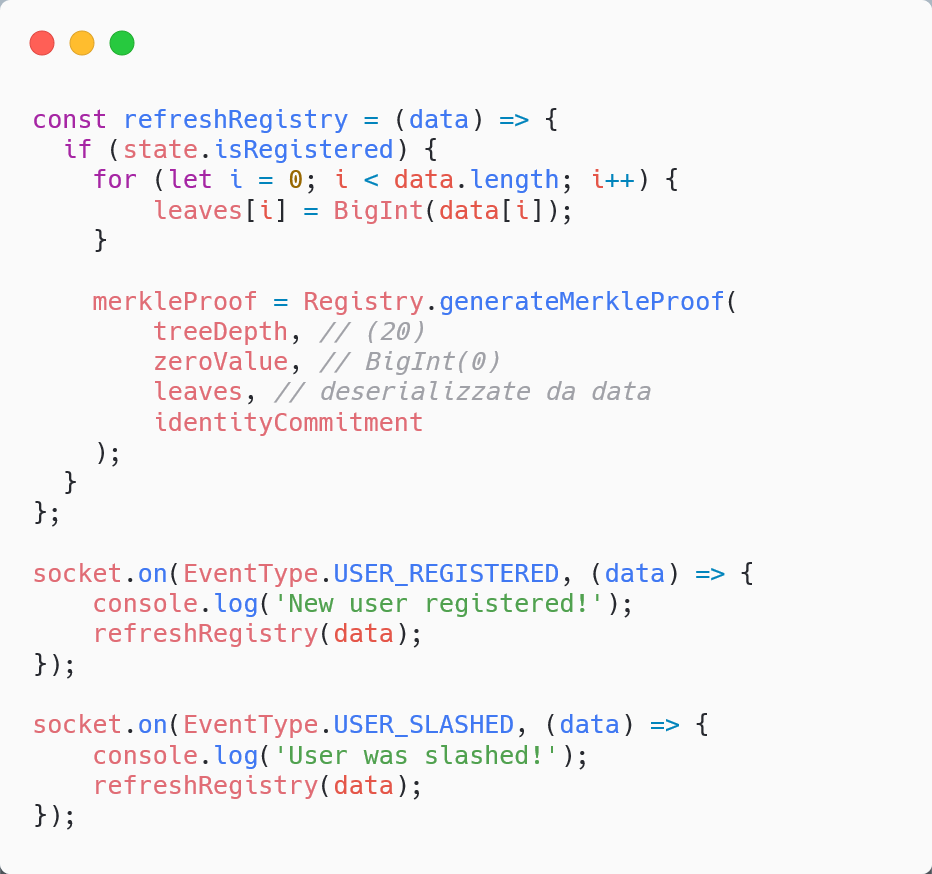
\includegraphics[width=10cm]{./chapters/3.poc/images/4.1.client.png}
    \label{fig:1.client}
    \captionsetup{justification=centering}
    \caption{codice Client sincronizzazione registri}
\end{figure}
Per ottimizzare la fase di interazione la generazione della prova di appartenenza al registro viene effettuata ad ogni sincronizzazione.
La fase di registrazione è abbastanza banale in quanto è costituita solamente dall'invio dell'identity commitment al server a dall'attesa del relativo aknowledgement. Mentre la fase di interazione è più articolata in quanto è durante questa fase che il Client genera la prova di appartenere all'albero e di avere generato le porzioni di chiave da rilascaire in modo corretto. In questa fase, per testare le funzionalità di rate limiting, ho incluso la possibilità per l'utente di selezionare l'opzione "dos". Grazie a questa opzione, l'utente potrà provare ad inviare 100 messaggi nello stesso intervallo di tempo. Prima d'interagire con il sistema l'utente genera una prova utilizzando il segnale, che una volta applicata la funzione hash rappresenterà la nostra cordinata $x$, la merkleProof e l'externalNullifier. Le altre infomazioni necessarie come la chiave privata o l'rln\_identifier vengono ricavate da un istanza della libreria RLNjs creata durante le fasi iniziali del Client.\clearpage
\begin{figure}[H]
    \centering
    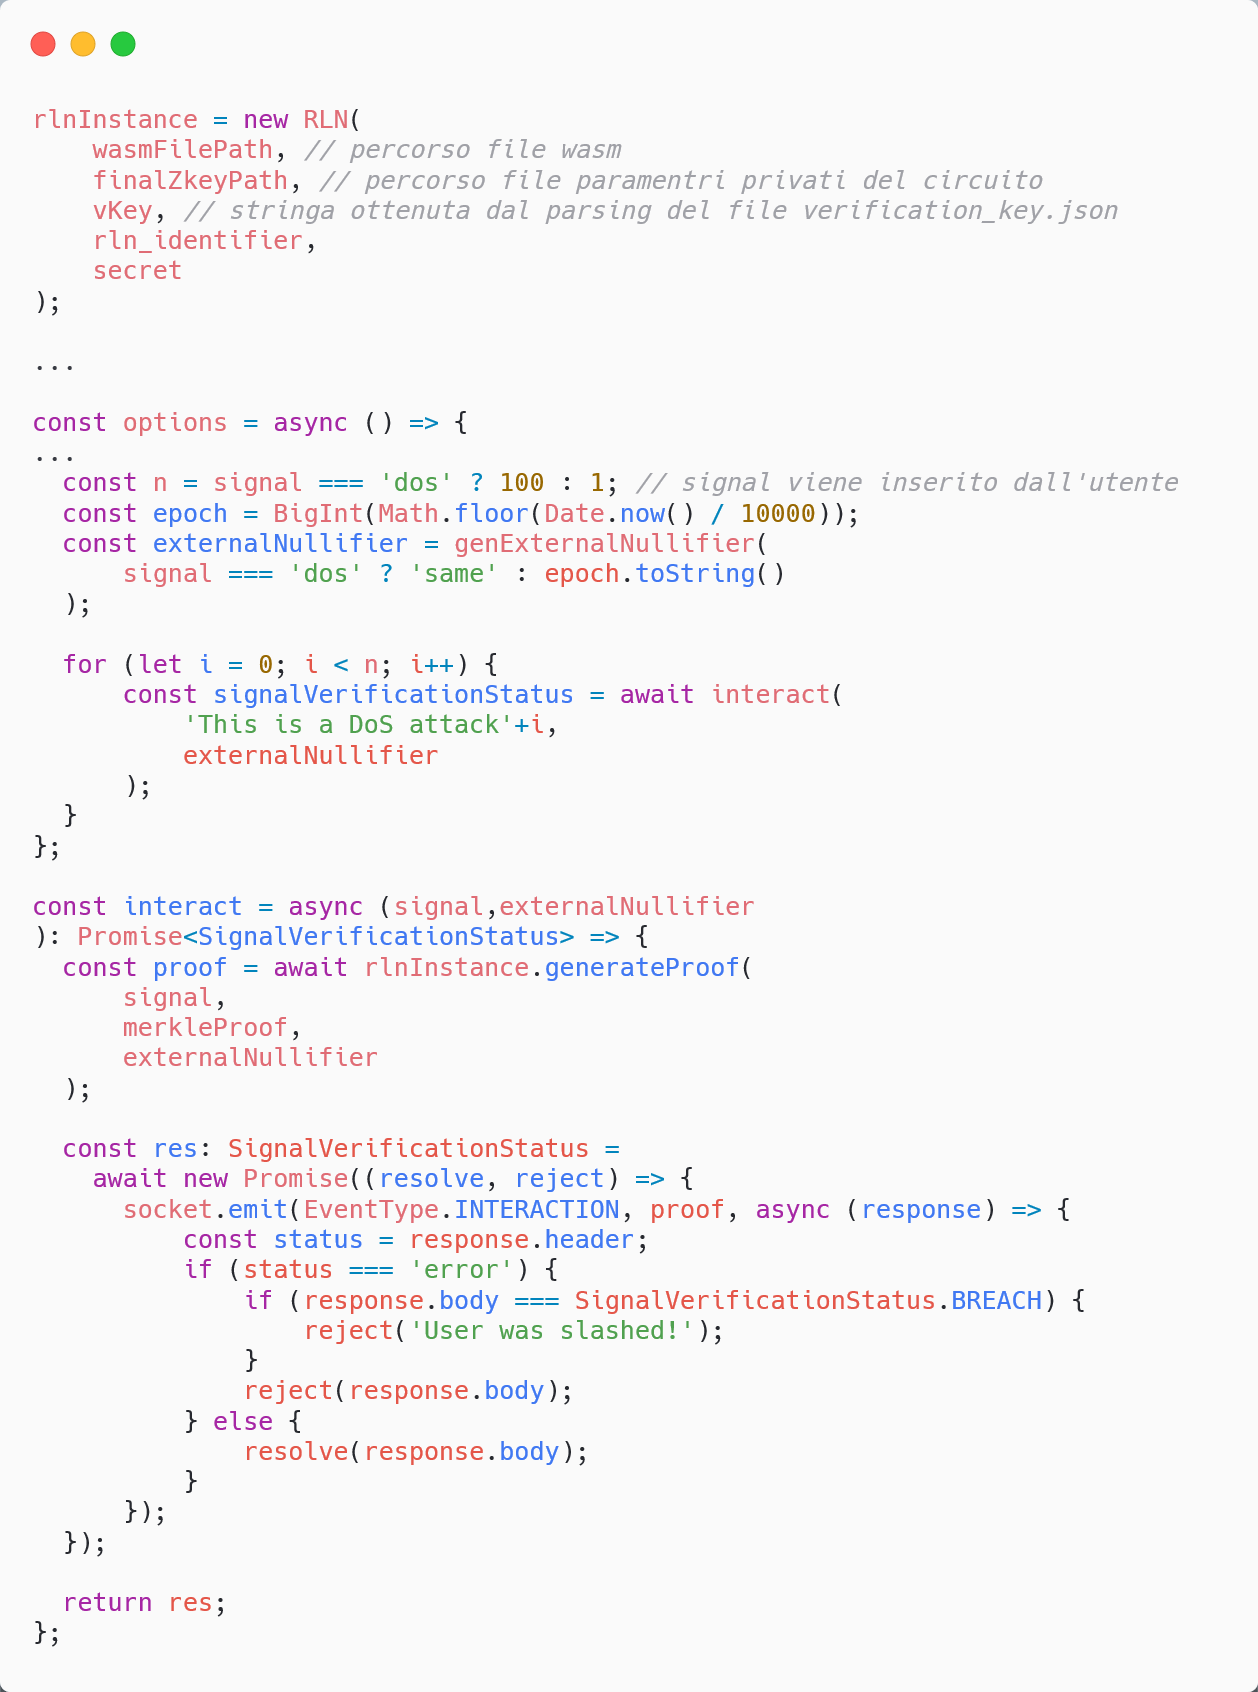
\includegraphics[width=11cm]{./chapters/3.poc/images/4.2.client.png}
    \label{fig:2.client}
    \captionsetup{justification=centering}
    \caption{codice Client interazione con il sistema}
\end{figure}

\section{Prestazioni}
Di seguito riporto alcuni dati significativi ottenuti dall'esecuzione del prototipo. I test sono stati effettuati su un computer con le seguenti caratteristiche:
\begin{itemize}
    \item CPU: Apple silicon M1
    \item RAM: 8GB
    \item OS: MacOS Ventura 13.0
\end{itemize}

Inizieremo analizzando il numero di vincoli che costituiscono i circuiti per la generazione delle prove e le loro dimensioni. È importante ricordare che i circuiti sono stati generati utilizzando la libreria Circom 2. Per i test che verranno presentati, sono state utilizzate tre diverse profondità degli alberi di Merkle: 16, 24 e 32, che corrispondono rispettivamente ad un massimo di $2^{16}$, $2^{24}$ e $2^{32}$ utenti.
\begin{figure}[H]
    \centering
    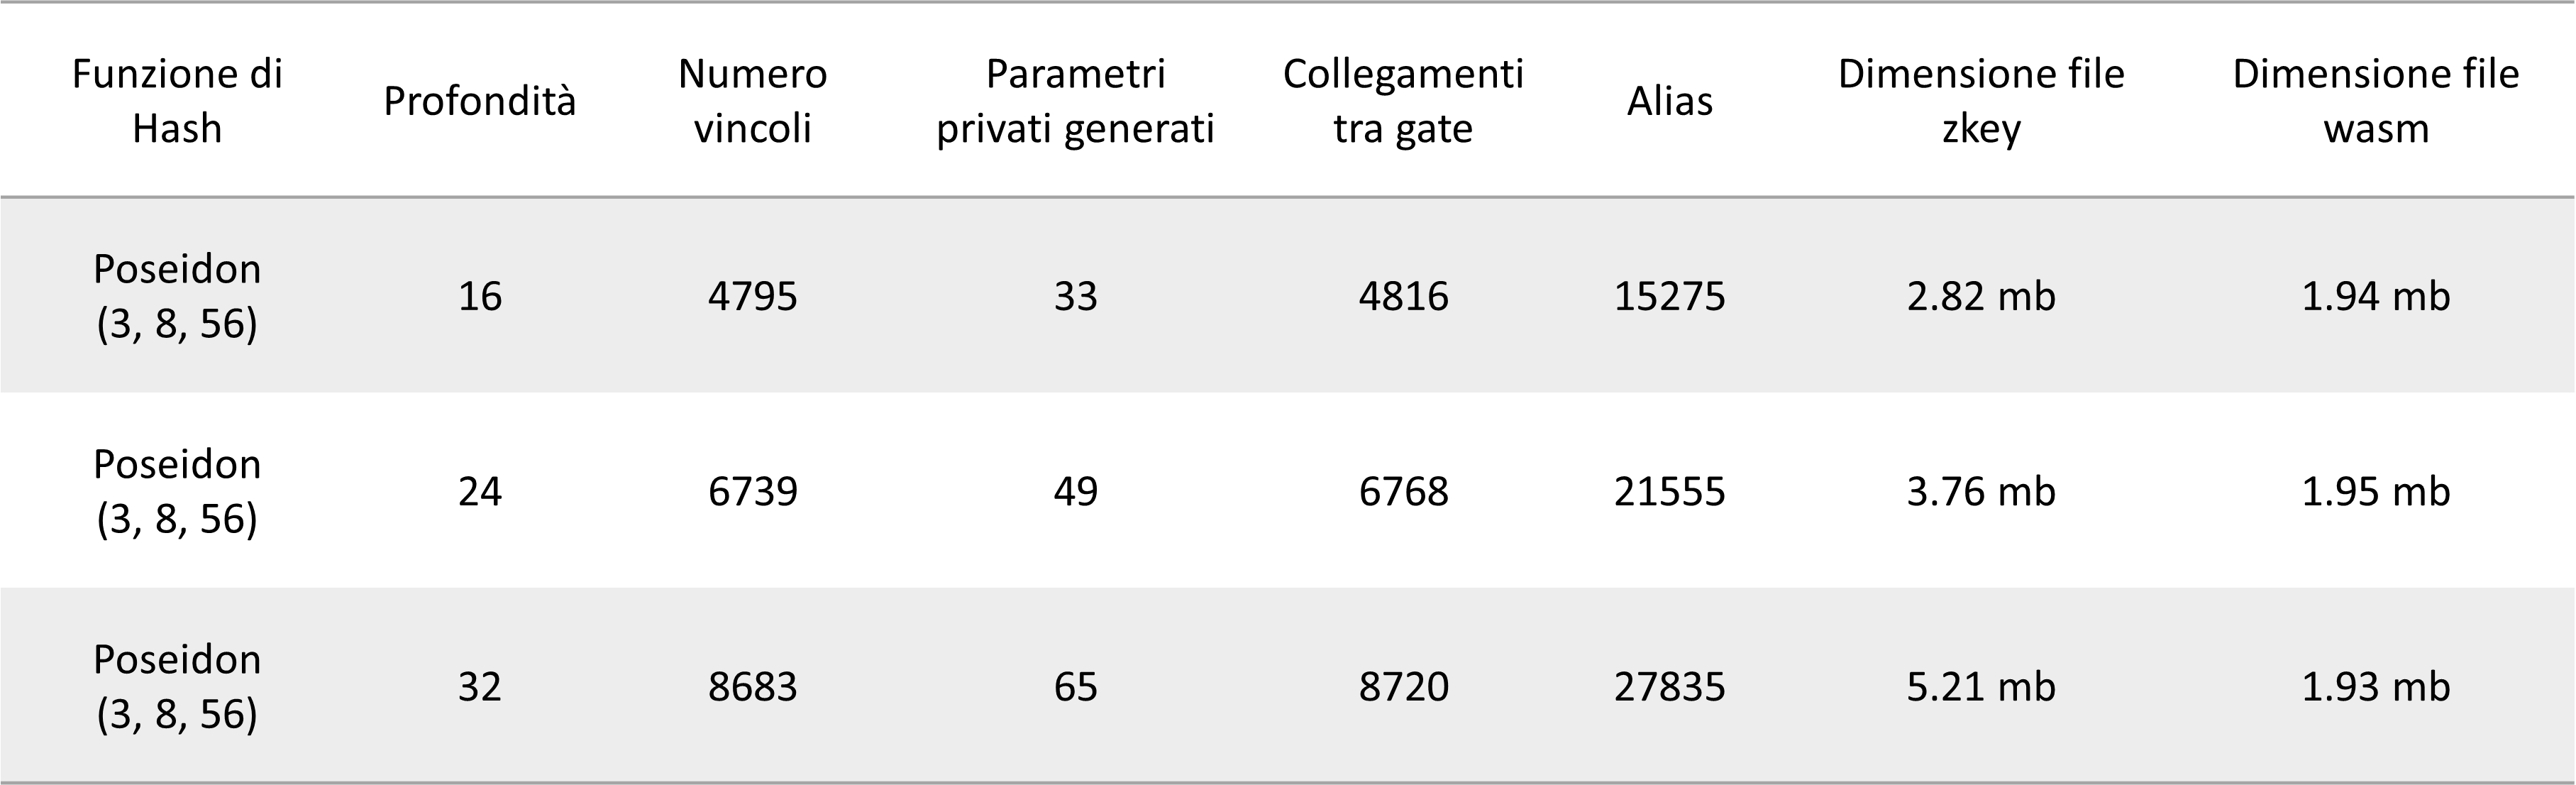
\includegraphics[width=17cm]{./chapters/3.poc/images/5.1.bench.png}
    \label{fig:1.bench}
    \captionsetup{justification=centering}
    \caption{codice Client interazione con il sistema}
\end{figure}
I dati più significativi sono il numero di vincoli, le dimensioni dei file rln\_final.zkey e rln.wasm. Infatti, se a un primo impatto i numeri dei vincoli generati dai circuiti possono sembrare molto elevati, in realtà le dimensioni dei file sono notevolemente ridotte, se pensiamo che un albero di Merkle di profondità 30 utilizzando una funzione di hash con output 128 bit, può arrivare pesare decine di GB. Di seguito invece mostriamo i tempi di esecuzione:
\begin{figure}[H]
    \centering
    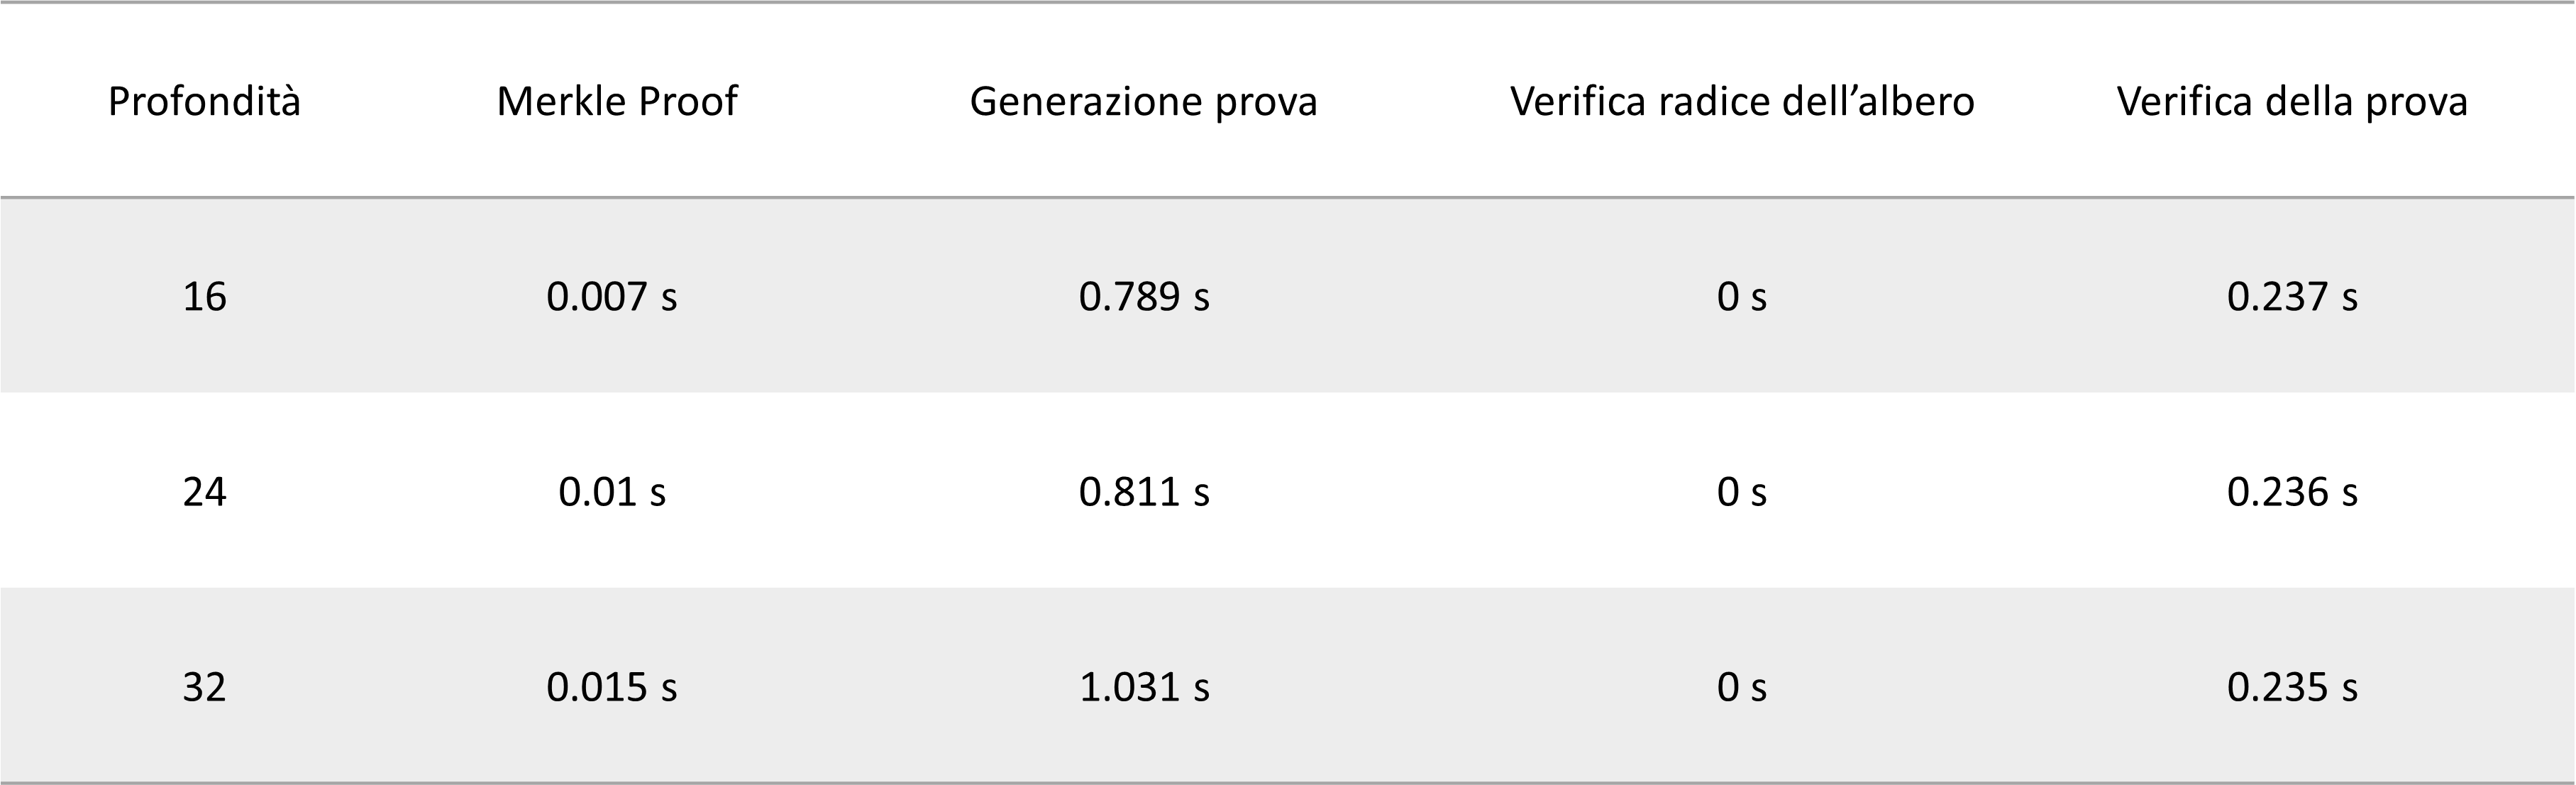
\includegraphics[width=17cm]{./chapters/3.poc/images/5.2.bench.png}
    \label{fig:2.bench}
    \captionsetup{justification=centering}
    \caption{codice Client interazione con il sistema}
\end{figure}

qui i dati più significativi sono i tempi di generazione e verifica delle prove, in particolare la verifica che rimane praticamente costante. La colonna con indice "Verifica radice dell'albero" rappresenta la velocità con cui il sistema riesce a verificare se la radice dell'albero con cui è stata generata la prova è uguale a quello correto.